

\section{OpticalElement: \textquotedbl{}MICADO\textquotedbl{}%
  \label{opticalelement-micado}%
}

\textbf{Element}: instrument

\textbf{Alias}: INST

\textbf{Description}: Effects from the MICADO common optics


\subsection{Global properties%
  \label{global-properties}%
}

\begin{quote}
\begin{alltt}
\begin{lstlisting}[frame=single]
       temperature : -190
filter_file_format : filters/TC_filter_\{\}.dat
      element_name : MICADO
\end{lstlisting}
\end{alltt}
\end{quote}


\subsection{Effects%
  \label{effects}%
}

Summary of Effects included in this optical element:

\setlength{\DUtablewidth}{\linewidth}
\begin{longtable*}[c]{|p{0.098\DUtablewidth}|p{0.272\DUtablewidth}|p{0.284\DUtablewidth}|p{0.110\DUtablewidth}|p{0.191\DUtablewidth}|}
\hline
\textbf{%
element
} & \textbf{%
name
} & \textbf{%
class
} & \textbf{%
included
} & \textbf{%
z\_orders
} \\
\hline
\endfirsthead
\hline
\textbf{%
element
} & \textbf{%
name
} & \textbf{%
class
} & \textbf{%
included
} & \textbf{%
z\_orders
} \\
\hline
\endhead
\multicolumn{5}{c}{\hfill ... continued on next page} \\
\endfoot
\endlastfoot

MICADO
 & 
micado\_static\_surfaces
 & 
SurfaceList
 & 
True
 & 
{[}20, 120, 520{]}
 \\
\hline

MICADO
 & 
micado\_ncpas\_psf
 & 
NonCommonPathAberration
 & 
True
 & 
{[}241, 641{]}
 \\
\hline

MICADO
 & 
filter\_wheel\_1
 & 
FilterWheel
 & 
True
 & 
{[}124, 224, 524{]}
 \\
\hline

MICADO
 & 
filter\_wheel\_2
 & 
FilterWheel
 & 
True
 & 
{[}124, 224, 524{]}
 \\
\hline

MICADO
 & 
pupil\_wheel
 & 
FilterWheel
 & 
True
 & 
{[}124, 224, 524{]}
 \\
\hline
\end{longtable*}
\label{tbl-micado}


\subsubsection{SurfaceList: \textquotedbl{}micado\_static\_surfaces\textquotedbl{}%
  \label{surfacelist-micado-static-surfaces}%
}

\textbf{Included by default}: \texttt{True}

\textbf{File Description}: surfaces list for wide field optics

\textbf{Class Description}: <no docstring>

\textbf{Changes}:

\begin{itemize}
\item 2019-01-28 (KL) Changed column names and added units to header

\item 2019-07-10 (KL) Shortened the list to only the swappable mirrors

\item 2020-08-25 (KL) Updated angle\_unit to degree from degrees (why has astropy not complained until now?)

\item 2020-10-10 (KL) Added SCAO pick-off dichroic after CM17 conversation
\end{itemize}


\paragraph{Data%
  \label{data}%
}

\begin{figure}[H]
\noindent\makebox[\linewidth][c]{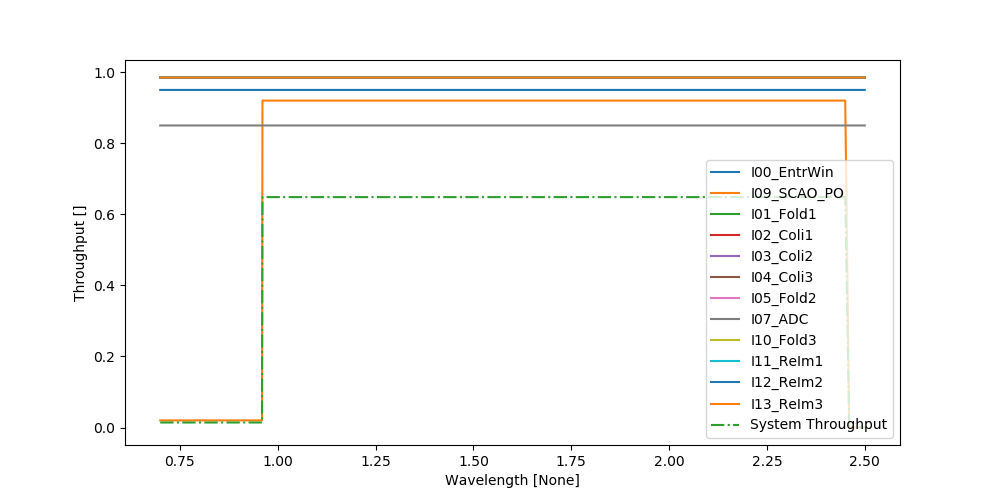
\includegraphics{micado_static_surfaces.png}}\phantomsection\label{fig-micado-static-surfaces}
\end{figure}

\setlength{\DUtablewidth}{\linewidth}
\begin{longtable*}[c]{|p{0.145\DUtablewidth}|p{0.075\DUtablewidth}|p{0.075\DUtablewidth}|p{0.075\DUtablewidth}|p{0.145\DUtablewidth}|p{0.156\DUtablewidth}|p{0.284\DUtablewidth}|}
\hline
\textbf{%
name
} & \textbf{%
outer
} & \textbf{%
inner
} & \textbf{%
angle
} & \textbf{%
temperature
} & \textbf{%
action
} & \textbf{%
filename
} \\
\hline
\endfirsthead
\hline
\textbf{%
name
} & \textbf{%
outer
} & \textbf{%
inner
} & \textbf{%
angle
} & \textbf{%
temperature
} & \textbf{%
action
} & \textbf{%
filename
} \\
\hline
\endhead
\multicolumn{7}{c}{\hfill ... continued on next page} \\
\endfoot
\endlastfoot

I00\_EntrWin
 & 
0.5
 & 
0.0
 & 
0
 & 
0
 & 
transmission
 & 
TER\_entrance\_window.dat
 \\
\hline

I09\_SCAO\_PO
 & 
0.5
 & 
0.0
 & 
45
 & 
-190
 & 
reflection
 & 
TER\_SCAO\_dichroic.dat
 \\
\hline

I01\_Fold1
 & 
0.5
 & 
0.0
 & 
45
 & 
-190
 & 
reflection
 & 
TER\_mirror\_gold.dat
 \\
\hline

I02\_Coli1
 & 
0.4
 & 
0.0
 & 
10
 & 
-190
 & 
reflection
 & 
TER\_mirror\_gold.dat
 \\
\hline

I03\_Coli2
 & 
0.2
 & 
0.0
 & 
10
 & 
-190
 & 
reflection
 & 
TER\_mirror\_gold.dat
 \\
\hline

I04\_Coli3
 & 
0.2
 & 
0.0
 & 
10
 & 
-190
 & 
reflection
 & 
TER\_mirror\_gold.dat
 \\
\hline

I05\_Fold2
 & 
0.2
 & 
0.0
 & 
45
 & 
-190
 & 
reflection
 & 
TER\_mirror\_gold.dat
 \\
\hline

I07\_ADC
 & 
0.2
 & 
0.0
 & 
0
 & 
-190
 & 
transmission
 & 
TER\_full\_adc.dat
 \\
\hline

I10\_Fold3
 & 
0.2
 & 
0.0
 & 
45
 & 
-190
 & 
reflection
 & 
TER\_mirror\_gold.dat
 \\
\hline

I11\_ReIm1
 & 
0.2
 & 
0.0
 & 
10
 & 
-190
 & 
reflection
 & 
TER\_mirror\_gold.dat
 \\
\hline

I12\_ReIm2
 & 
0.2
 & 
0.0
 & 
10
 & 
-190
 & 
reflection
 & 
TER\_mirror\_gold.dat
 \\
\hline

I13\_ReIm3
 & 
0.2
 & 
0.0
 & 
10
 & 
-190
 & 
reflection
 & 
TER\_mirror\_gold.dat
 \\
\hline
\end{longtable*}
\label{tbl-micado-static-surfaces}


\paragraph{Meta-data%
  \label{meta-data}%
}

\begin{quote}
\begin{alltt}
\begin{lstlisting}[frame=single]
            filename : LIST_MICADO_mirrors_static.dat
                name : micado_static_surfaces
         temperature : -190
  filter_file_format : filters/TC_filter_\{\}.dat
        element_name : MICADO
              author : Kieran Leschinski
              source : Ric's SPIE 2018 PPT presentation
        date_created : 2018-11-19
       date_modified : 2019-07-10
              status : Design, pre PDR list of all static MICADO surfaces
                type : mirror:list
          outer_unit : m
          inner_unit : m
          angle_unit : degree
    temperature_unit : deg_C
             z_order : [20, 120, 520]
             include : True
        ignore_wings : False
            wave_min : !SIM.spectral.wave_min
            wave_max : !SIM.spectral.wave_max
           wave_unit : !SIM.spectral.wave_unit
            wave_bin : !SIM.spectral.spectral_resolution
 report_plot_include : True
report_table_include : True
  minimum_throughput : !SIM.spectral.minimum_throughput
             etendue : !TEL.etendue
\end{lstlisting}
\end{alltt}
\end{quote}


\subsubsection{NonCommonPathAberration: \textquotedbl{}micado\_ncpas\_psf\textquotedbl{}%
  \label{noncommonpathaberration-micado-ncpas-psf}%
}

\textbf{Included by default}: \texttt{True}

\textbf{File Description}: Effective NCPA induced PSF kernel

\textbf{Class Description}: Needed: pixel\_scale

\textbf{Changes}:

\begin{itemize}
\item 2018-11-19 (KL) updated meta data to new format
\end{itemize}


\paragraph{Data%
  \label{id1}%
}

\begin{figure}[H]
\noindent\makebox[\linewidth][c]{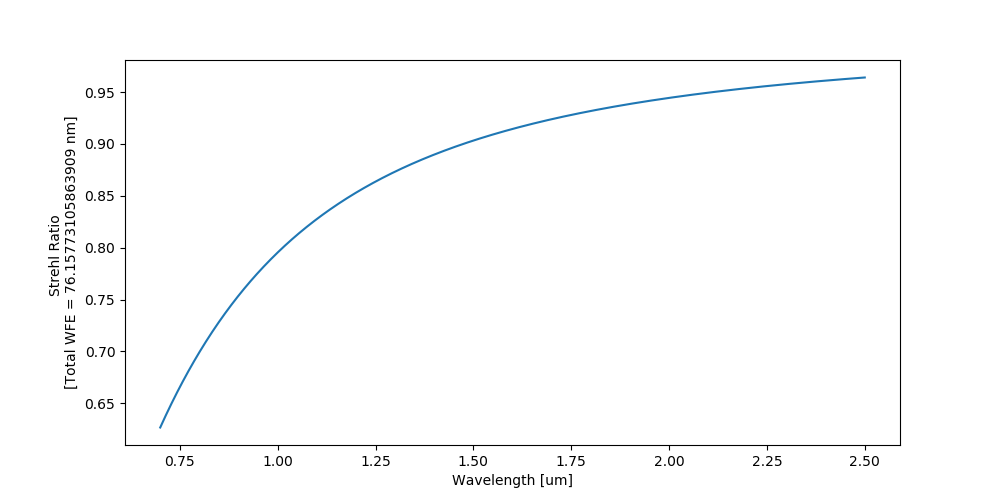
\includegraphics{micado_ncpas_psf.png}}\phantomsection\label{fig-micado-ncpas-psf}
\end{figure}


\paragraph{Meta-data%
  \label{id2}%
}

\begin{quote}
\begin{alltt}
\begin{lstlisting}[frame=single]
            filename : INST_MICADO_wavefront_error_budget.dat
                name : micado_ncpas_psf
         temperature : -190
  filter_file_format : filters/TC_filter_\{\}.dat
        element_name : MICADO
         pixel_scale : 0.004
              author : Kieran Leschinski
             sources : Ric Davies email
        date_created : 2016-11-21
       date_modified : 2018-11-19
                type : instrument:wavefront_errors_list
              status : Idea - based on the WFE budget and emails with Ric
        wfe_rms_unit : nm
             z_order : [241, 641]
             include : True
       flux_accuracy : 0.001
      sub_pixel_flag : False
       convolve_mode : full
            wave_key : WAVE0
    normalise_kernel : True
 report_plot_include : True
report_table_include : False
        kernel_width : None
        strehl_drift : 0.02
            wave_min : !SIM.spectral.wave_min
            wave_max : !SIM.spectral.wave_max
\end{lstlisting}
\end{alltt}
\end{quote}


\subsubsection{FilterWheel: \textquotedbl{}filter\_wheel\_1\textquotedbl{}%
  \label{filterwheel-filter-wheel-1}%
}

\textbf{Included by default}: \texttt{True}

\textbf{File Description}:

\textbf{Class Description}: Examples

\textbf{Changes}:

\begin{itemize}
\item \end{itemize}


\paragraph{Data%
  \label{id3}%
}

\begin{figure}[H]
\noindent\makebox[\linewidth][c]{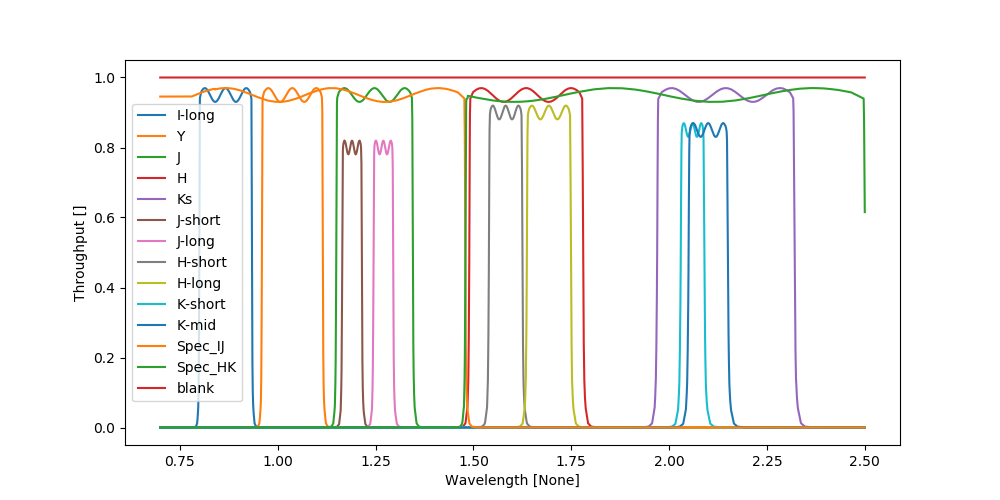
\includegraphics{filter_wheel_1.png}}\phantomsection\label{fig-filter-wheel-1}
\end{figure}

\setlength{\DUtablewidth}{\linewidth}
\begin{longtable*}[c]{|p{0.098\DUtablewidth}|p{0.086\DUtablewidth}|p{0.086\DUtablewidth}|p{0.145\DUtablewidth}|p{0.133\DUtablewidth}|}
\hline
\textbf{%
name
} & \textbf{%
\begin{description}
\item[{centre}] \leavevmode 
um

\end{description}
} & \textbf{%

\begin{description}
\item[{width}] \leavevmode 
um

\end{description}
} & \textbf{%
\begin{description}
\item[{blue cutoff}] \leavevmode 
um

\end{description}
} & \textbf{%
\begin{description}
\item[{red cutoff}] \leavevmode 
um

\end{description}
} \\
\hline
\endfirsthead
\hline
\textbf{%
name
} & \textbf{%
\begin{description}
\item[{centre}] \leavevmode 
um

\end{description}
} & \textbf{%
\begin{description}
\item[{width}] \leavevmode 
um

\end{description}
} & \textbf{%
\begin{description}
\item[{blue cutoff}] \leavevmode 
um

\end{description}
} & \textbf{%
\begin{description}
\item[{red cutoff}] \leavevmode 
um

\end{description}
} \\
\hline
\endhead
\multicolumn{5}{c}{\hfill ... continued on next page} \\
\endfoot
\endlastfoot

I-long
 & 
0.8689
 & 
0.1340
 & 
0.8019
 & 
0.9359
 \\
\hline

Y
 & 
1.0396
 & 
0.1550
 & 
0.9621
 & 
1.1171
 \\
\hline

J
 & 
1.2502
 & 
0.1950
 & 
1.1527
 & 
1.3477
 \\
\hline

H
 & 
1.6395
 & 
0.2900
 & 
1.4945
 & 
1.7845
 \\
\hline

Ks
 & 
2.1500
 & 
0.3500
 & 
1.9750
 & 
2.3250
 \\
\hline

J-short
 & 
1.1902
 & 
0.0490
 & 
1.1657
 & 
1.2147
 \\
\hline

J-long
 & 
1.2702
 & 
0.0490
 & 
1.2457
 & 
1.2947
 \\
\hline

H-short
 & 
1.5830
 & 
0.0850
 & 
1.5405
 & 
1.6255
 \\
\hline

H-long
 & 
1.6937
 & 
0.1120
 & 
1.6377
 & 
1.7497
 \\
\hline

K-short
 & 
2.0602
 & 
0.0600
 & 
2.0302
 & 
2.0902
 \\
\hline

K-mid
 & 
2.1005
 & 
0.1000
 & 
2.0505
 & 
2.1505
 \\
\hline

Spec\_IJ
 & 
1.1663
 & 
0.6990
 & 
0.8168
 & 
1.5158
 \\
\hline

Spec\_HK
 & 
2.0345
 & 
1.0200
 & 
1.5245
 & 
2.5445
 \\
\hline

blank
 & 
2.7545
 & 
2.7000
 & 
1.4045
 & 
4.1045
 \\
\hline
\end{longtable*}
\label{tbl-filter-wheel-1}


\paragraph{Meta-data%
  \label{id4}%
}

\begin{quote}
\begin{alltt}
\begin{lstlisting}[frame=single]
             filename : None
                 name : filter_wheel_1
          temperature : -190
   filter_file_format : filters/TC_filter_\{\}.dat
         element_name : MICADO
         filter_names : ['I-long', 'Y', 'J', 'H', 'Ks', 'J-short', 'J-long', 'H-short', 'H-long', 'K-short', 'K-mid', 'Spec_IJ', 'Spec_HK', 'blank']
      filename_format : !INST.filter_file_format
       current_filter : !OBS.filter_name_fw1
   minimum_throughput : 0.000101
                outer : 0.2
           outer_unit : m
              z_order : [124, 224, 524]
              include : True
                 path :
  report_plot_include : True
 report_table_include : True
report_table_rounding : 4
\end{lstlisting}
\end{alltt}
\end{quote}


\subsubsection{FilterWheel: \textquotedbl{}filter\_wheel\_2\textquotedbl{}%
  \label{filterwheel-filter-wheel-2}%
}

\textbf{Included by default}: \texttt{True}

\textbf{File Description}:

\textbf{Class Description}: Examples

\textbf{Changes}:

\begin{itemize}
\item \end{itemize}


\paragraph{Data%
  \label{id5}%
}

\begin{figure}[H]
\noindent\makebox[\linewidth][c]{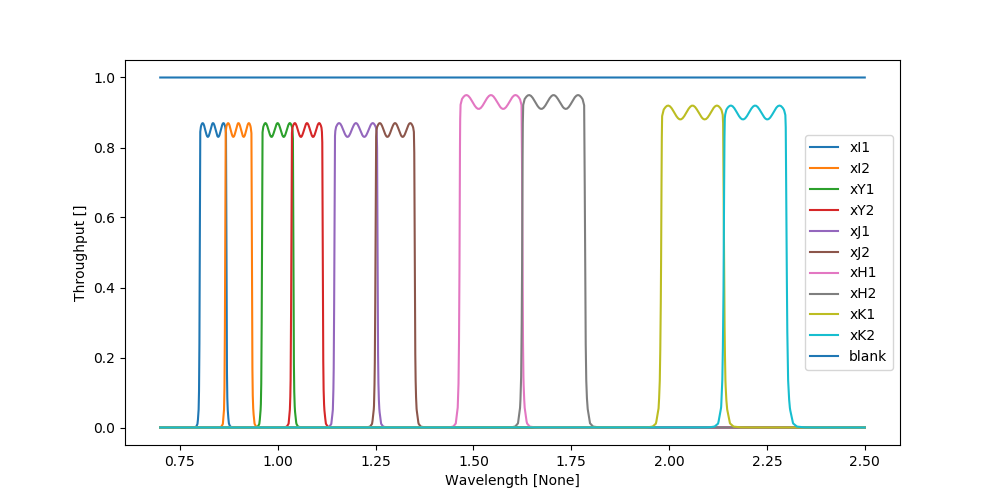
\includegraphics{filter_wheel_2.png}}\phantomsection\label{fig-filter-wheel-2}
\end{figure}

\setlength{\DUtablewidth}{\linewidth}
\begin{longtable*}[c]{|p{0.075\DUtablewidth}|p{0.086\DUtablewidth}|p{0.086\DUtablewidth}|p{0.145\DUtablewidth}|p{0.133\DUtablewidth}|}
\hline
\textbf{%
name
} & \textbf{%
\begin{description}
\item[{centre}] \leavevmode 
um

\end{description}
} & \textbf{%
\begin{description}
\item[{width}] \leavevmode 
um

\end{description}
} & \textbf{%
\begin{description}
\item[{blue cutoff}] \leavevmode 
um

\end{description}
} & \textbf{%
\begin{description}
\item[{red cutoff}] \leavevmode 
um

\end{description}
} \\
\hline
\endfirsthead
\hline
\textbf{%
name
} & \textbf{%
\begin{description}
\item[{centre}] \leavevmode 
um

\end{description}
} & \textbf{%
\begin{description}
\item[{width}] \leavevmode 
um

\end{description}
} & \textbf{%
\begin{description}
\item[{blue cutoff}] \leavevmode 
um

\end{description}
} & \textbf{%
\begin{description}
\item[{red cutoff}] \leavevmode 
um

\end{description}
} \\
\hline
\endhead
\multicolumn{5}{c}{\hfill ... continued on next page} \\
\endfoot
\endlastfoot

xI1
 & 
0.8355
 & 
0.0680
 & 
0.8015
 & 
0.8695
 \\
\hline

xI2
 & 
0.9005
 & 
0.0680
 & 
0.8665
 & 
0.9345
 \\
\hline

xY1
 & 
1.0006
 & 
0.0800
 & 
0.9606
 & 
1.0406
 \\
\hline

xY2
 & 
1.0756
 & 
0.0800
 & 
1.0356
 & 
1.1156
 \\
\hline

xJ1
 & 
1.2009
 & 
0.1100
 & 
1.1459
 & 
1.2559
 \\
\hline

xJ2
 & 
1.3007
 & 
0.1000
 & 
1.2507
 & 
1.3507
 \\
\hline

xH1
 & 
1.5465
 & 
0.1600
 & 
1.4665
 & 
1.6265
 \\
\hline

xH2
 & 
1.7064
 & 
0.1600
 & 
1.6264
 & 
1.7864
 \\
\hline

xK1
 & 
2.0612
 & 
0.1600
 & 
1.9812
 & 
2.1412
 \\
\hline

xK2
 & 
2.2211
 & 
0.1600
 & 
2.1411
 & 
2.3011
 \\
\hline

blank
 & 
2.7545
 & 
2.7000
 & 
1.4045
 & 
4.1045
 \\
\hline
\end{longtable*}
\label{tbl-filter-wheel-2}


\paragraph{Meta-data%
  \label{id6}%
}

\begin{quote}
\begin{alltt}
\begin{lstlisting}[frame=single]
             filename : None
                 name : filter_wheel_2
          temperature : -190
   filter_file_format : filters/TC_filter_\{\}.dat
         element_name : MICADO
         filter_names : ['xI1', 'xI2', 'xY1', 'xY2', 'xJ1', 'xJ2', 'xH1', 'xH2', 'xK1', 'xK2', 'blank']
      filename_format : !INST.filter_file_format
       current_filter : !OBS.filter_name_fw2
   minimum_throughput : 0.000101
                outer : 0.2
           outer_unit : m
              z_order : [124, 224, 524]
              include : True
                 path :
  report_plot_include : True
 report_table_include : True
report_table_rounding : 4
\end{lstlisting}
\end{alltt}
\end{quote}


\subsubsection{FilterWheel: \textquotedbl{}pupil\_wheel\textquotedbl{}%
  \label{filterwheel-pupil-wheel}%
}

\textbf{Included by default}: \texttt{True}

\textbf{File Description}:

\textbf{Class Description}: Examples

\textbf{Changes}:

\begin{itemize}
\item \end{itemize}


\paragraph{Data%
  \label{id7}%
}

\begin{figure}[H]
\noindent\makebox[\linewidth][c]{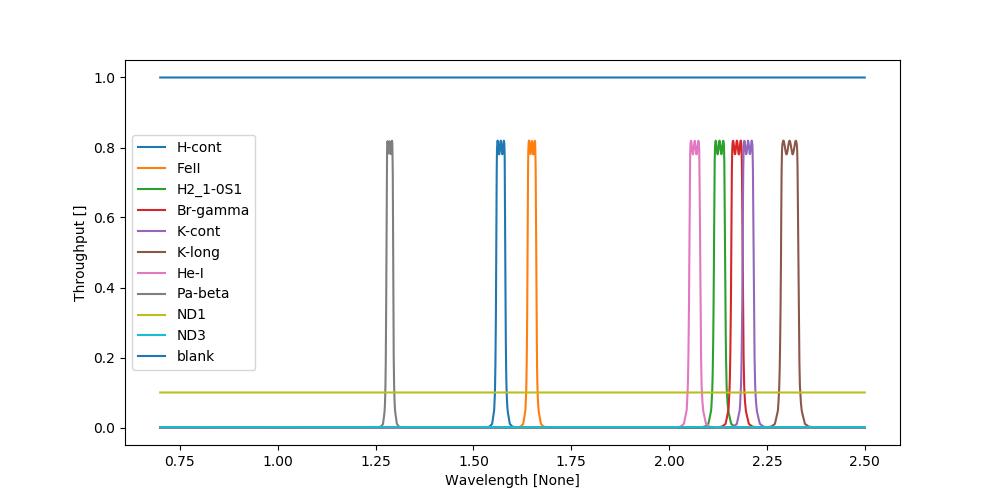
\includegraphics{pupil_wheel.png}}\phantomsection\label{fig-pupil-wheel}
\end{figure}

\setlength{\DUtablewidth}{\linewidth}
\begin{longtable*}[c]{|p{0.110\DUtablewidth}|p{0.086\DUtablewidth}|p{0.086\DUtablewidth}|p{0.145\DUtablewidth}|p{0.133\DUtablewidth}|}
\hline
\textbf{%
name
} & \textbf{%
\begin{description}
\item[{centre}] \leavevmode 
um

\end{description}
} & \textbf{%
\begin{description}
\item[{width}] \leavevmode 
um

\end{description}
} & \textbf{%
\begin{description}
\item[{blue cutoff}] \leavevmode 
um

\end{description}
} & \textbf{%
\begin{description}
\item[{red cutoff}] \leavevmode 
um

\end{description}
} \\
\hline
\endfirsthead
\hline
\textbf{%
name
} & \textbf{%
\begin{description}
\item[{centre}] \leavevmode 
um

\end{description}
} & \textbf{%
\begin{description}
\item[{width}] \leavevmode 
um

\end{description}
} & \textbf{%
\begin{description}
\item[{blue cutoff}] \leavevmode 
um

\end{description}
} & \textbf{%
\begin{description}
\item[{red cutoff}] \leavevmode 
um

\end{description}
} \\
\hline
\endhead
\multicolumn{5}{c}{\hfill ... continued on next page} \\
\endfoot
\endlastfoot

H-cont
 & 
1.5701
 & 
0.0220
 & 
1.5591
 & 
1.5811
 \\
\hline

FeII
 & 
1.6495
 & 
0.0210
 & 
1.6390
 & 
1.6600
 \\
\hline

H2\_1-0S1
 & 
2.1289
 & 
0.0280
 & 
2.1149
 & 
2.1429
 \\
\hline

Br-gamma
 & 
2.1734
 & 
0.0280
 & 
2.1594
 & 
2.1874
 \\
\hline

K-cont
 & 
2.2019
 & 
0.0270
 & 
2.1884
 & 
2.2154
 \\
\hline

K-long
 & 
2.3081
 & 
0.0440
 & 
2.2861
 & 
2.3301
 \\
\hline

He-I
 & 
2.0656
 & 
0.0270
 & 
2.0521
 & 
2.0791
 \\
\hline

Pa-beta
 & 
1.2865
 & 
0.0170
 & 
1.2780
 & 
1.2950
 \\
\hline

ND1
 & 
2.7529
 & 
0.0000
 & 
2.7529
 & 
2.7529
 \\
\hline

ND3
 & 
2.7529
 & 
0.0000
 & 
2.7529
 & 
2.7529
 \\
\hline

blank
 & 
2.7545
 & 
2.7000
 & 
1.4045
 & 
4.1045
 \\
\hline
\end{longtable*}
\label{tbl-pupil-wheel}


\paragraph{Meta-data%
  \label{id8}%
}

\begin{quote}
\begin{alltt}
\begin{lstlisting}[frame=single]
             filename : None
                 name : pupil_wheel
          temperature : -190
   filter_file_format : filters/TC_filter_\{\}.dat
         element_name : MICADO
         filter_names : ['H-cont', 'FeII', 'H2_1-0S1', 'Br-gamma', 'K-cont', 'K-long', 'He-I', 'Pa-beta', 'ND1', 'ND3', 'blank']
      filename_format : !INST.filter_file_format
       current_filter : !OBS.filter_name_pupil
   minimum_throughput : 0.000101
                outer : 0.2
           outer_unit : m
              z_order : [124, 224, 524]
              include : True
                 path :
  report_plot_include : True
 report_table_include : True
report_table_rounding : 4
\end{lstlisting}
\end{alltt}
\end{quote}
